\chapter{Background: Interatomic Potential Fitting}

\begin{changemargin}{1.0cm}{1.0cm}
\abstractpreamble{It is known that Chromium is }
\end{changemargin}




\FloatBarrier
\section{Experiment, Modelling and Theory}

\FloatBarrier
\subsection{Introduction}


Experiment: direct answers from physical reality
Limited by technology of the time, also limits due to Heisenberg uncertainty principle
Theory: state of the art theories have been replaced numerous times in the past
Quantum mechanics is a very accurate theory under certain circumstances
Some problems just too hard to solve with these theories
Modelling: bridges the gap
Experiment and theory have their flaws, so does modelling
Helps show what experiment can’t, and where theory is too hard to solve
Aim: take very accurate DFT calculations based on quantum theory, extrapolate to a larger scale by fitting EAM potentials, open a path to simulations of Pd + Fe and Ru + Fe



\begin{figure}[htbp]
  \begin{center}
    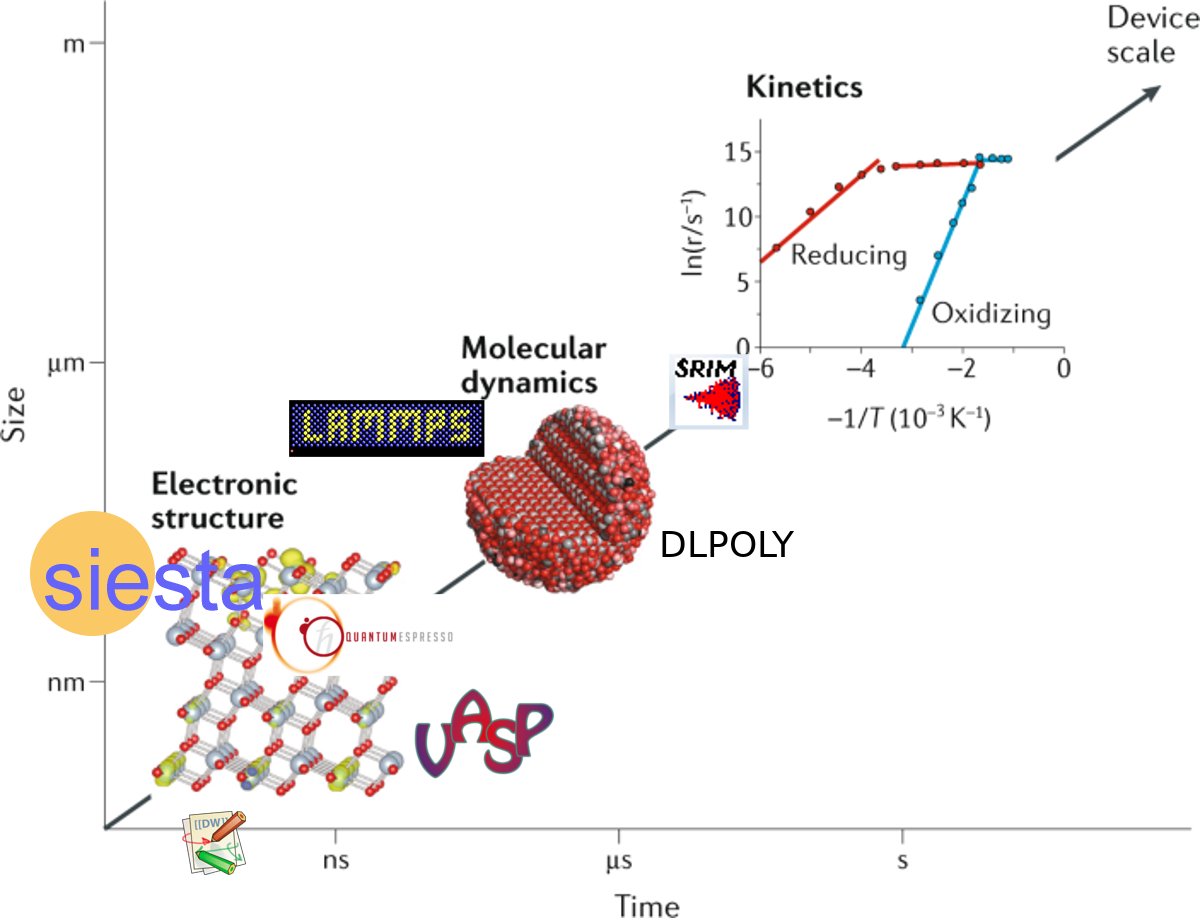
\includegraphics[width=10.0cm]{chapters/background_potential_fitting/images/scale.png}
    \captionsetup{font={it}}
    \caption{Time and Size Scales for Computer Packages \cite{scalediagram}}
    \label{fig:electricityusagesuk}
  \end{center}
\end{figure}



\FloatBarrier
\subsection{Simulating Materials on a Variety of Scales in Time and Space}

Stainless steel grain size less than 100 microns.  A 1 micron grain would contain tens of billions of atoms.  Given this number of atoms for a very small grain, it is very difficult to simulate just one grain over a short time period.

Certain properties derived ab initio assume the entire material is a single crystal, rather than made from grains of crystals.  





































